\documentclass[]{article}
\usepackage{amsmath}
\usepackage{amsthm}
\usepackage{amssymb}
\usepackage{graphicx}
\usepackage[utf8]{inputenc} 
\usepackage{subcaption}
\usepackage{caption}
\usepackage{hyperref}
\usepackage{amsbsy}
\usepackage[left=4cm]{geometry}
 %http://tex.stackexchange.com/questions/595/how-can-i-get-bold-math-symbols
%opening
\title{Variance reduction in coarse bifurcation analysis of stochastic models}
\author{Pieter Van Nuffel}

\newcommand{\R}{\ensuremath{\mathbb{R}}} % commando zonder argumenten
\newcommand{\C}{\ensuremath{\mathbb{C}}}
\newcommand{\N}{\ensuremath{\mathbb{N}}}
\newcommand{\E}{\ensuremath{\mathbb{E}}}
\newcommand{\norm}[1]{\left\|#1\right\|} % commando's met argumenten
\newcommand{\pa}[2]{\frac{\partial #1}{\partial #2}}
\newcommand{\ppa}[2]{\frac{\partial^2 #1}{\partial #2^2}}
\newcommand{\dd}{\ensuremath{\mathrm{d}}}
\newcommand{\U}{\ensuremath{\boldsymbol{\rho}}}
\newcommand{\cts}{\ensuremath{\boldsymbol{\Phi}^N_T}} %Coarse time step
\newcommand{\V}{\ensuremath{\mathbf{v}}} 
\newcommand{\jv}{\ensuremath{\mathbf{\hat{Jv}}}}
\newcommand{\jvpde}{\ensuremath{\mathbf{Jv}_{FP}}}

\theoremstyle{definition}
\newtheorem{Theorem}{Theorem}


\begin{document}

\maketitle{}

\begin{abstract}


In this project, we develop a Newton-Krylov method that is able to compute efficiently coarse fixed points when the underlying fine-scale dynamics is stochastic. We investigate the use of correlated samples to perform a more accurate approximation of the Jacobian vector products that are needed in a Krylov solution in each Newton iteration. The main novelty of the algorithm is in the elimination of the noise that is generated when estimating Jacobian-vector products using time-integration of perturbed initial conditions. We present numerical results that demonstrate the convergence properties of the numerical method, and use the method to show   the emergence of coarse equilibrium state





%system of diffusion processes have a stabilizing force acting on each of them, corresponding to a bistable potential.



%nd use the method to show that macroscopic
%fronts in this model destabilise at a coarse symmetry-breaking bifurcation.
%
%We consider a system of diffusion processes that interact through their empirical mean and have a stabilizing force acting on each of them, corresponding to a bistable potential. There are three parameters that characterize the system: the strength of the intrinsic stabilization, the strength of the external random perturbations, and the degree of cooperation or interaction between them. The latter is the rate of mean reversion of each component to the empirical mean of the system. We interpret this model in the context of systemic risk and analyze in detail the effect of cooperation between the components, that is, the rate of mean reversion. We show that in a certain regime of parameters increasing cooperation tends to increase the stability of the individual agents but it also increases the overall or systemic risk. We use the theory of large deviations of diffusions interacting through their mean field.
%
%
%The present paper thus contains two main contributions. First, for the specific
%system under study, we explain the birth of the above-described macroscopic states in
%terms of coarse symmetry-breaking bifurcations. To the best of our knowledge, steps
%in this direction were taken only very recently [55, 7] and were confined to globally
%locked-in states. In the homogeneous case, we follow [5] and interpret metastable
%locked-in states as fixed points of a coarse evolution map. In the limit of infinitely
%many globally-coupled agents with homogeneous product preferences, we derive the
%coarse evolution map analytically. In the case of heterogeneous agents we employ
%stochastic continuation and show for the first time how fronts destabilise to partially
%locked-in states.
%The second main contribution of the paper is the development of a novel procedure
%to obtain coarse Jacobian-vector products with reduced variance, allowing
%the accurate evaluation of Jacobian-vector products in the presence of microscopic
%stochasticity, thus gaining full control over the linear and the nonlinear iterations
%of the Newton-Krylov solver. Even though our implementation of variance-reduced
%Jacobian-vector products is specific to the lock-in model, we believe that analogous
%strategies can be applied to other ABMs. Therefore, we provide a detailed account of
%the algorithmic steps involved in defining an accurate equation-free Newton-Krylov
%method and testing its convergence properties


\end{abstract}

 
\section{Model problem}



\subsection{Advection-diffusion}

In general, we are interested in performing a bifurcation analysis for  models at which an exact, closed model at the macroscopic level is not available. However, as a toy problem, we start using an example where the macroscopic model is already known. On the macroscopic scale the evolution of a probability density $\rho$ is given by a PDE of the advection-diffusion type

\begin{equation} 
\label{fokkerplanck}
\pa{\rho(x,t)}{t} + \mu \pa{(f(x) \rho(x,t))}{x} = \frac{\sigma^2}{2}  \ppa{\rho(x,t)}{x} .
\end{equation}

The advection represents gradient-driven flow, according to an advection coefficient $\mu$ and a force $f(x) = - \pa {V}{x}$. In this example $V(x)$ is chosen to be a bi-stable potential $V(x) = x^4-x^2$. 
The microscopic model consists in simulating an ensemble of $N$ particles evolving according to the corresponding SDE
\begin{equation} 
\label{SDE}
     \dd \mathbf{X_t} = \mu f(\mathbf{X_t}) \dd t + \sigma \dd{\mathbf{W_t}},
\end{equation}
where $\mathbf{W_t}$ are $N$ independent, standard Brownian motions.



\subsection{Discretization}

We look for solutions of the Fokker-Planck-equation \eqref{fokkerplanck}
in two ways:
\begin{itemize}
\item By explicitly solving eq. \eqref{fokkerplanck} using the discretization scheme
\begin{equation} 
\label{pde_discretization}
\rho_i^{n+1} = \rho_i^n + \Delta t \left( \frac{\sigma^2}{2{\Delta x}^2} \left( \rho_{i+1}^{n} - 2 \rho_i^n + \rho_{i-1}^n \right)  - \mu \frac{f(x)}{\Delta x} (\rho_i^n - \rho_{i-1}^n) \right)
\end{equation}
for the value  of $\rho$ at position $x=i \Delta x$ and time $t=(n+1) \Delta t$. This is a first-order upwind scheme for the advective part combined with the Forward-Time Central-Space-method for the diffusive part.


\item By simulating an ensemble of $N$ particles evolving according to the SDE \label{SDE}.  The position $X^{n+1}$ of each  particle  at time $t= (n+1) \Delta t$ is simulated using the Euler-Maruyama scheme
\begin{equation}
   X^{n + 1} = X^{n} + \mu f(X^n) \Delta t +  \sigma \sqrt{\Delta t}\cdot \xi^n \label{Euler-Mar}
\end{equation}
with $\xi^n  \sim \mathcal{N} (0,1)$.
\end{itemize}

%
%
%\section{Convergence of variance-reduced Jacobian-vector-products}
%
%
%\subsection{Why do we need variance reduction of the Jacobian-vector products?  \label{section:Jv}}
%
%
%
%If we want to compute steady states for the density $\U_*$ without direct simulation, we can find them by solving the non-linear system
%
%\begin{equation}
%  \U_* - \cts(\U_*) =0.
%\end{equation}
%In each Newton iteration, one needs to solve a linear system involving the Jacobian of \cts, denoted as $D(\cts)$.  Since we do not have an explicit formula for
%$D(\cts)$ we are forced to use an iterative method (such as GMRES) that only
%requires Jacobian-vector products. 
%The Jacobian $D(\cts)$ applied to a vector $\mathbf{v}$ (with unit norm) will be estimated by a finite difference approximation
%\begin{eqnarray}
%\label{Jv_approx}
%D(\cts) \cdot \mathbf{v} &\approx& \frac{\cts (\U + \varepsilon \mathbf{v}, \boldsymbol{\omega_1} )  - \cts (\U, \boldsymbol{\omega_2})}{\varepsilon} \\
%&\approx & \frac{\cts (\U, \boldsymbol{\omega_1} )  + \varepsilon D(\cts) (  \U, \boldsymbol{\omega_1})  \cdot \mathbf{v}  - \cts (\U, \boldsymbol{\omega_2}) }{\varepsilon} \nonumber
%.
%\end{eqnarray}
%
%If we use the solution of the PDE, eq. \eqref{pde_discretization}, the time stepper is deterministic and the calculation of the Jacobian-vector products is straightforward. If we use the solutions of the SDE however, we have to deal with numerical noise in evaluating eq. \ref{Jv_approx}.
%Because the coarse time-stepper is stochastic, repeating $\cts$ with two sets of random numbers $\boldsymbol{\omega_1},  \boldsymbol{\omega_2}$  will give different results. For $ \varepsilon \ll 1$ this will result in an $\mathcal{O}(1/(\varepsilon^2 N))$ variance. Consequently the variance on the Jacobian-vector-products will grow unboundedly as $\varepsilon$ tends to zero and $D(\cts) \cdot \mathbf{v}$ completely loses the structure of the perturbation \V.
%
%\subsection{How do we reduce the variance of the Jacobian-vector products?}
%This numerical noise can be reduced by using the same random numbers $\boldsymbol{\omega}$ for the unperturbed and perturbed simulations. If we apply the weighted restriction operator \eqref{restriction_eps},  we get the same microscopic realizations in the lifting step - the only difference is in the computation of the weights. As such,  we impose $\boldsymbol{\omega_1} = \boldsymbol{\omega_2}$ in eq. \eqref{Jv_approx} and consequently
%the variance of $D(\cts) \cdot \mathbf{v}$ is bounded and of  $\mathcal{O}(1/ N)$.  Fig. \ref{Var_N} shows that the variance on the stochastic solution for the Jacobian-vector-product converges to zero with $\mathcal{O}(1/ N)$ and that it does not depend on the value of $\varepsilon$.

%\begin{figure}
%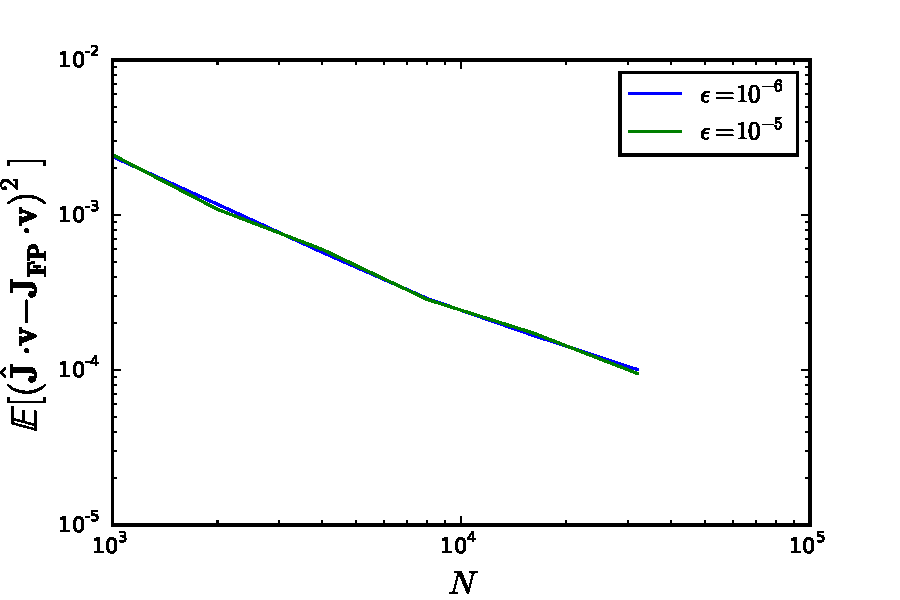
\includegraphics{../results/plots/ms_Jveps-5eps-6}
%\caption{}
%\label{Convergence_Jv}
%\end{figure}



%\subsection{Results}
%
%From now on, let us abbreviate the Jacobian-vector product $D(\cts) \cdot \mathbf{v}$  estimated from the for particle-based time-stepper as $\jv$.  We also chose the perturbation vector $\V$ to be sinusiodal  (the convergence plots will be  independent from $\V$). If we calculate $\jv$ from the stochastic simulations with different number of particles $N$, we can test two things: the convergence to zero of the variance on $\jv$ and the convergence to zero of the estimated bias on $\jv$.  We will also plot the mean squared error (MSE) which incorporates both effects (see eq. \eqref{MSE}. 
%The bias can be estimated by comparing the expectation value $\norm{\jv}$ with the Jacobian-vector product for the PDE solved on a fine grid, denoted as $\jvpde$. The estimated expectation value $\mathbb{E}(\jv)$ is the Jacobian-vector averaged over $M$ stochastic simulations. 
%
%%\begin{equation} \label{MSE}
%%\texttt{MSE}(\jv, \mathbf{\bar{Jv} }) = \frac{ \mathbb{E} \left[   \left(  \jv - \mathbf{\bar{Jv}}  \right)^T  \cdot  \left(  \jv - \mathbf{\bar{Jv}}  \right) \right]} {n_x}  =    \texttt{Var}(\jv) +  \left( \texttt{Bias} (\jv)\right)^T \cdot  \left( \texttt{Bias} (\jv)\right)
%%\end{equation}
%%with 
%%\begin{equation} \nonumber
%% \texttt{Var}(\hat{Jv}) = \frac{ \mathbb{E} \left[   \left(  \jv - \mathbb{E}[\jv]   \right)^T  \cdot  \left(   \jv - \mathbb{E}[\jv]    \right) \right]} {n_x} 
%%\end{equation}
%
%
%\begin{equation} \label{MSE}
%\texttt{MSE}(\jv, \jvpde ) =  \mathbb{E} \left[   \left(  \jv - \jvpde  \right)^2 \right]  =   \texttt{Var}(\jv) +  \left( \mathbf{Bias}(\jv, \jvpde )  \right)^2
%\end{equation}
%with 
%\begin{equation} \label{Var}
% \texttt{Var}(\jv) =  \mathbb{E} \left[   \left(  \jv - \mathbb{E}[\jv]   \right)^2 \right] 
%\end{equation}
%and 
%\begin{equation} 
% \mathbf{Bias}(\jv, \jvpde ) = \mathbb{E}[\jv]  - \jvpde ,
%\end{equation}
%where we defined the inproduct of a $n_x$-dimensional vector $\V$ as $\mathbf{v}^2 = \frac{\V^T \cdot \V}{n_x}$. Thus, in eq. \eqref{MSE} and \eqref{Var} we divide by the number of discretization steps $n_x$ \footnote{If the number of discretisations steps for solving the PDE happens to be  higher than the number of bins $n_x$, we rescale the dimension of $\jvpde$ to $n_x$}. This allows us to make a meaningful comparison with solutions on finer or coarser grids. 
%
%
%
%%\begin{figure}
%%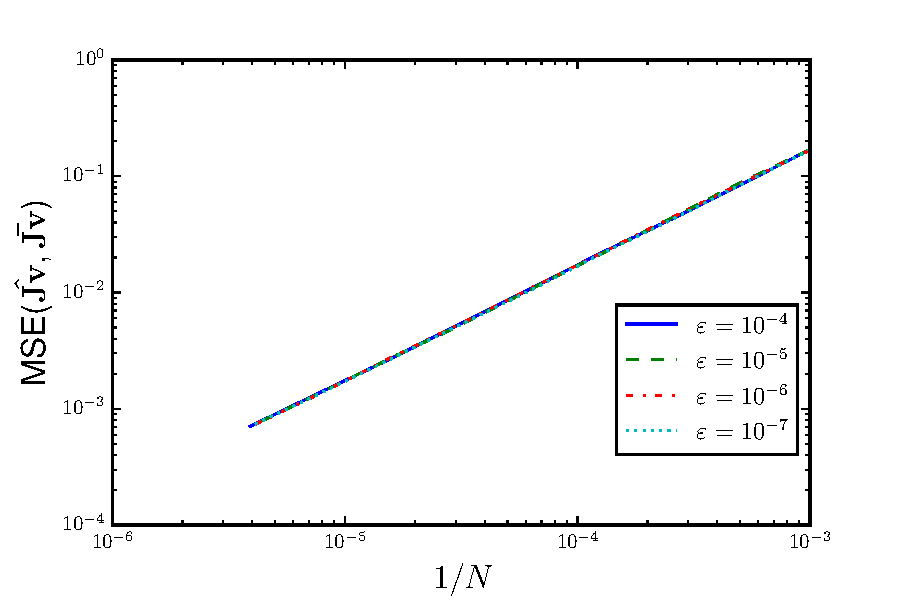
\includegraphics[width=14.5cm]{../Problems/WeightedParticles/checkSystem/plots/MSE_N_eps}
%%\caption{The mean squared error between the stochastic and the deterministic solution for the Jacobian-vector-product converges to zero with $\mathcal{O}(1/ N)$ and it does not depend on the value of $\varepsilon$.}
%%\label{MSE_N}
%%\end{figure}
%%
%\begin{figure}
%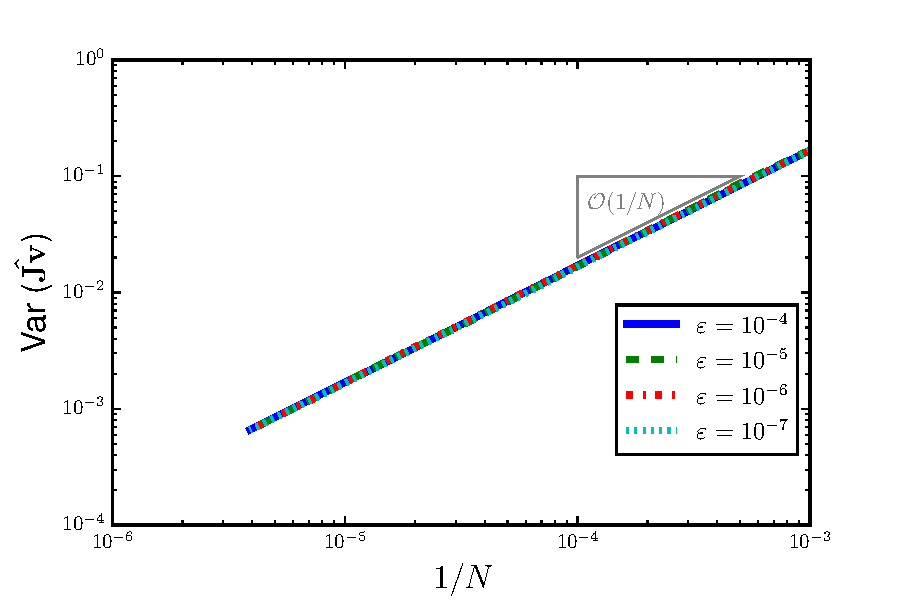
\includegraphics[width=14.5cm]{../Problems/WeightedParticles/checkSystem/plots/Var_N_eps}
%\caption{The variance on the stochastic solution for the Jacobian-vector-product converges to zero with $\mathcal{O}(1/ N)$ and it does not depend on the value of $\varepsilon$.}
%\label{Var_N}
%\end{figure}



%\begin{figure}
%\centering
%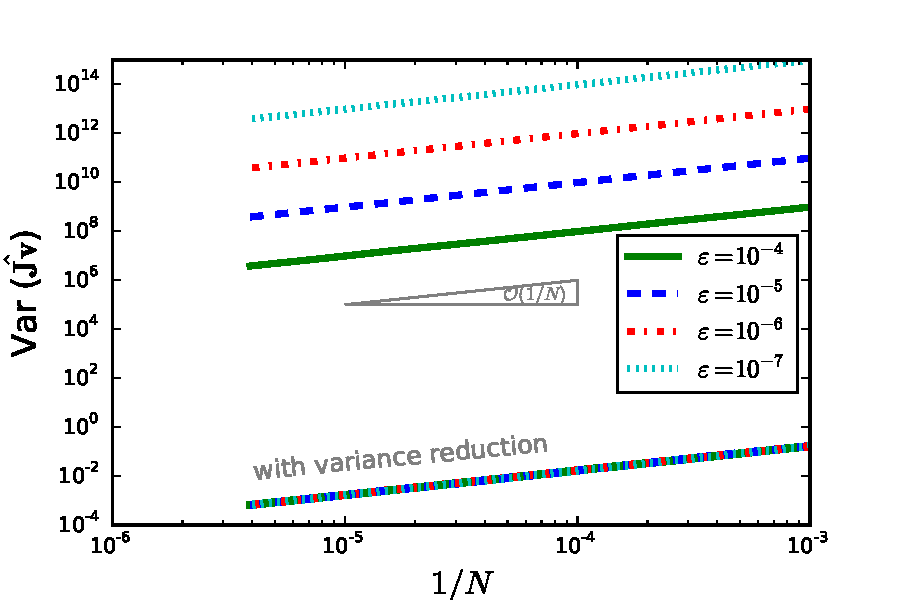
\includegraphics[width=0.8\linewidth]{../Problems/Particles/checkSystem/plots/Var_N_eps_nw}
%\caption[Effect of variance reduction]{In the case of unweighted restriction, the variance on the stochastic solution of the Jacobian-vector-product becomes unbounded as we decrease the perturbation size $\epsilon$. By using weights in the restriction step, the variance does not longer depend on the value of $\varepsilon$ and   converges to zero with $\mathcal{O}(1/ N)$.}
%\label{Var_N}
%\end{figure}


%
%%\begin{figure}
%%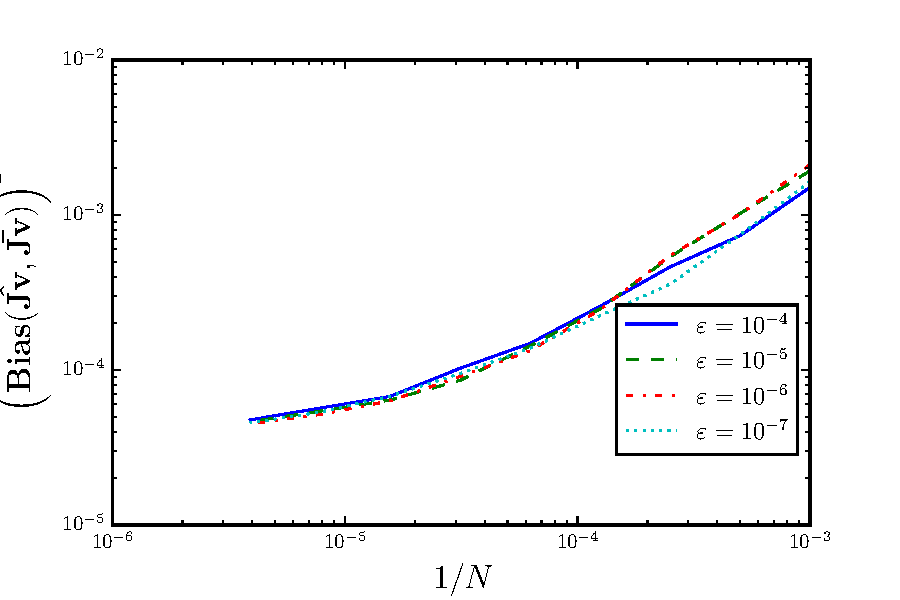
\includegraphics[width=14.5cm]{../Problems/WeightedParticles/checkSystem/plots/Bias_N_eps}
%%\caption{The squared bias between the stochastic and the deterministic solution for the Jacobian-vector-product does not depend on the value of $\varepsilon$.}
%%\label{Bias_N}
%%\end{figure}
%
%
%
%%
%%\begin{figure}
%%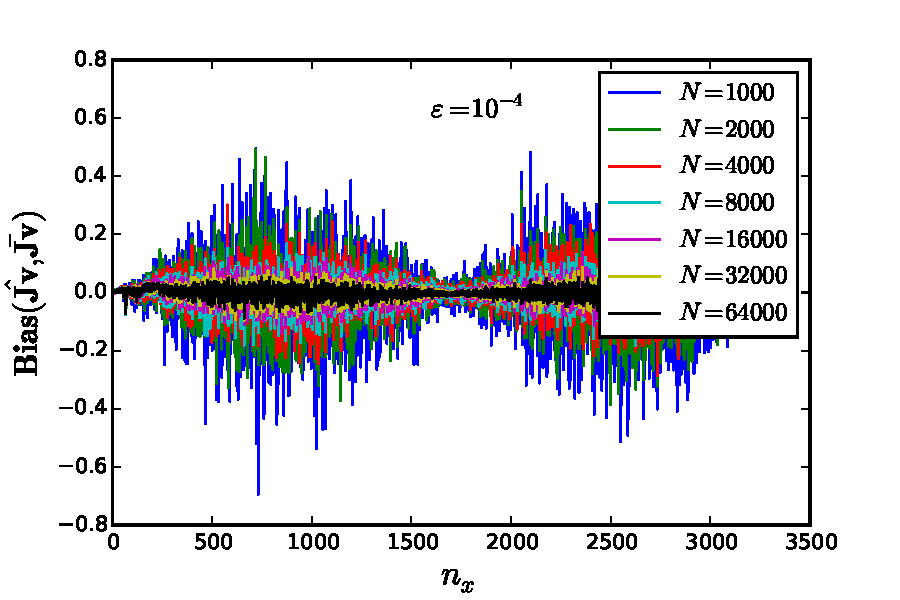
\includegraphics[width=8.5cm]{../Problems/WeightedParticles/checkSystem/plots/25-11Bias_e-_4}
%%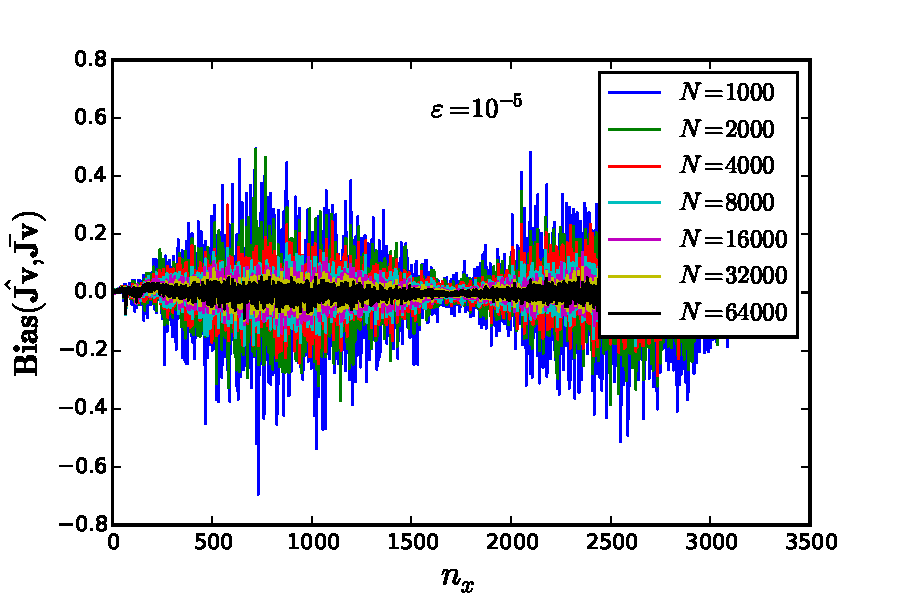
\includegraphics[width=8.5cm]{../Problems/WeightedParticles/checkSystem/plots/25-11Bias_e-_5}
%%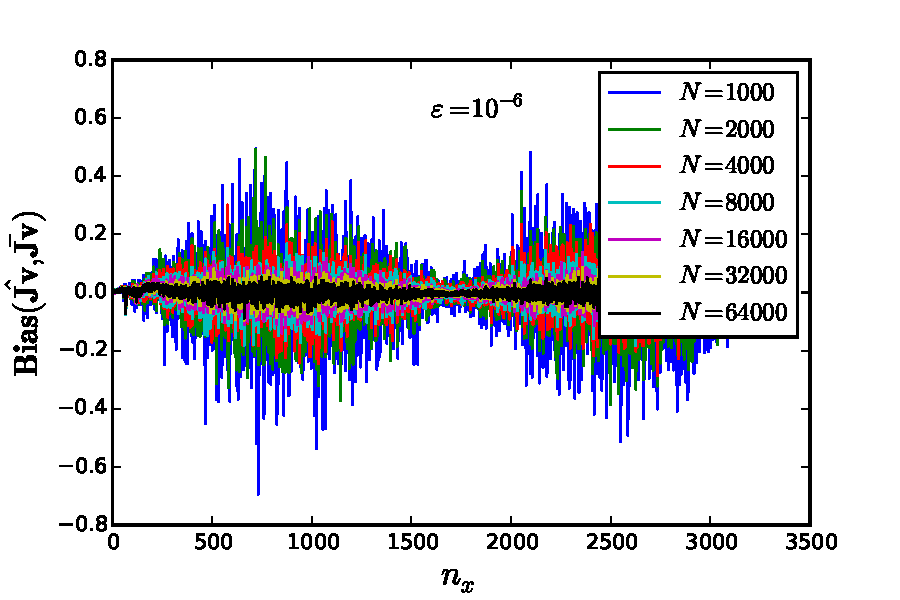
\includegraphics[width=8.5cm]{../Problems/WeightedParticles/checkSystem/plots/25-11Bias_e-_6}
%%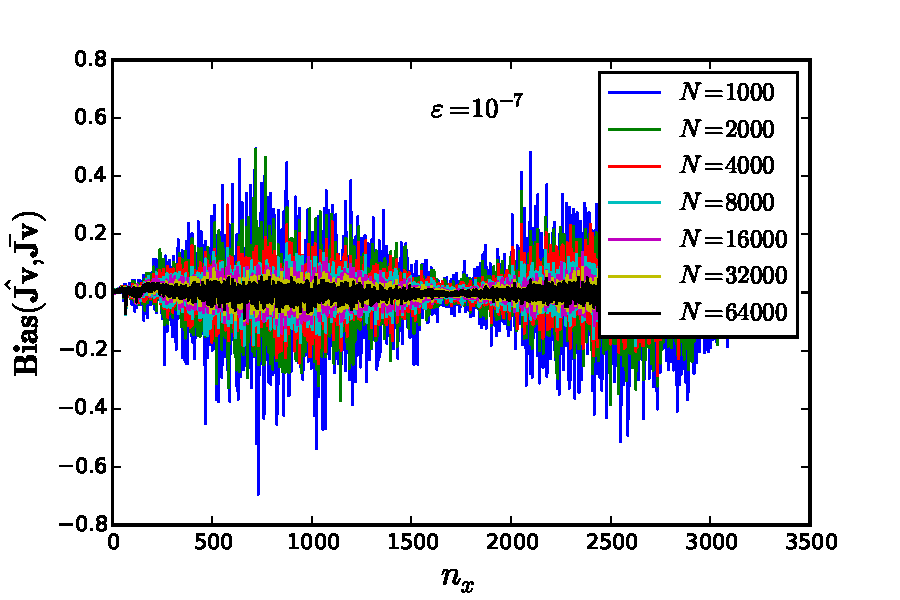
\includegraphics[width=8.5cm]{../Problems/WeightedParticles/checkSystem/plots/25-11Bias_e-_7}
%%\caption{The bias on the stochastic solution for the Jacobian-vector-product converges to zero if the number of particles is increased and it does not depend on the value of $\varepsilon$.}
%%\label{bias_v}
%%\end{figure}
%%
%
%
%
%
%
%\begin{table}
%
%\caption{Parameter values}
%   %FTCS-scheme  &   Euler-Maruyama-scheme  \\
% 
%     \begin{tabular} { | c  c | c | c |}    \hline   
%     %FTCS-scheme  &   Euler-Maruyama-scheme  \\  
%   \textit{ {Discretization parameters}}    &  & PDE  & SDE  \\ \hline
%    Discretization step  & $\Delta x $ & $10^{-4}$  & $10^{-2}$ \\ 
%        Number of discretization steps &  $n_x$ &  $34 000$ & 340 \\ 
%    Time step  &  $\Delta t$ & $10^{-8}$ &  $10^{-4}$ \\ 
%       Number of timesteps  & $n$  &  $10^{6}$ &  100   \\ \hline
%  \end{tabular}
%\quad
%     \begin{tabular}  { | c | c | c |  }  \hline
%     \multicolumn{3}{|c|} {\textit{ System parameters}   }    \\
%    \hline  
%    Diffusion coefficient  & $D $ & $0.5$ \\ 
%   Drift coefficient &  $a$ & $ 1$ \\ \hline
%  \multicolumn{3}{|c|} {\textit{ Simulation parameters}   }    \\ \hline
%   Number of realizations  & $M $ & $100$ \\ \hline
%    Perturbation size & $\varepsilon$  & $ 10^{-5}$ \\ \hline
%  \end{tabular}
%
%\end{table}
%
%
%
%
%%Total simulation time for particle-based time-stepper 
%%
%%Total Simulation time for PDE-based time stepper
%
%%\subsection{Variance}
%%\begin{equation}
%%\mathbb{E} \left[ (\rho -\mathbb{E}[\rho ])^2 \right] =?
%%\end{equation}
%%
%%
%%
%
%%\begin{equation}
%%D(\cts) \cdot \mathbf{v} \approx  \frac{\cts (\U, \boldsymbol{\omega_1} )  + \varepsilon \mathbf{v}  - \cts (\U, \boldsymbol{\omega_2}) }{\varepsilon} 
%%\end{equation}
%
%
%
%
%%\subsection{Convergence}
%
%%\section{Some documentation about the use of random numbers in the simulation}
%%
%%Every MC-step starts with a new seed for seeding the density sampler in the lifting step. This same seed is used for the time evolution of every particle. So, for a given MC-step and a given timestep, the brownian increment is the same for all particles in the simulation. This means that the sum of all Brownian steps is the same for all particles. This does not mean that $\Delta(x+\Delta T) - \Delta(x)$ is the same for all particles, because this depends on the drift-term, which depends on the position, which is different for every particle.
%
%
%\section{Convergence of the bias}
%We calculate the expectation value of $\jv$ by substituting eq. \eqref{} in the finite-difference approximation.
%
%\begin{equation}
%\E[\jv] =  \E \left[ \frac{\cts (\hat{\U} + \varepsilon \mathbf{v} )  - \cts (\hat{\U})}{\varepsilon}  \right]
%\end{equation}
%with \begin{equation}
%\cts (\hat{\U})  = \frac{1}{N}\sum_{i=1}^{N} \chi_{\Delta_j} \left[\mathcal{E} (x_i(t) \right]
%\end{equation}
%and 
%\begin{equation}
%\cts (\hat{\U} + \varepsilon \V )  = \frac{1}{N}\sum_{i=1}^{N}  (1+ \frac{\varepsilon \V}  {\U(x_i(t))}  ) \cdot \chi_{\Delta_j} \left[\mathcal{E} (x_i(t) \right] .
%\end{equation}
%
%
%\begin{eqnarray}
%\E[\jv] &=&  \E \left[  \frac{1}{N}\sum_{i=1}^{N}   \frac{ \chi_{\Delta_j} \left[  \mathcal{E} (x_i(t)) \right] \V}  {\U(x_i(t))}     \right] \\
%		&=&   \frac{\V}{N} \E \left[  \sum_{i=1}^{N}   \frac{ \chi_{\Delta_j} \left[  \mathcal{E} (x_i(t)) \right] }  {\U(x_i(t))}     \right] \\
%		&=&  \frac{\V}{N}  \sum_{i=1}^{N}   \frac{  \E \left[  \chi_{\Delta_j} \left[  \mathcal{E} (x_i(t)) \right]  \right] }  {\U(x_i(t))} \\
%		&=& \frac{\V}{N}  \sum_{i=1}^{N}   \frac{  \chi_{\Delta_j} \left[  \E \left[   \mathcal{E} (x_i(t)) \right]  \right] }  {\U(x_i(t))} 
%\end{eqnarray}
%
%
%
%%\begin{eqnarray}
%%\E[\jv] &=&  \E \left[ \frac{\cts (\hat{\U} + \varepsilon \mathbf{v} )  - \cts (\hat{\U})}{\varepsilon}  \right]
%%        &=&  \E \left[ \frac{1}{N} ] 
%%\end{eqnarray}
%
%\begin{figure}
%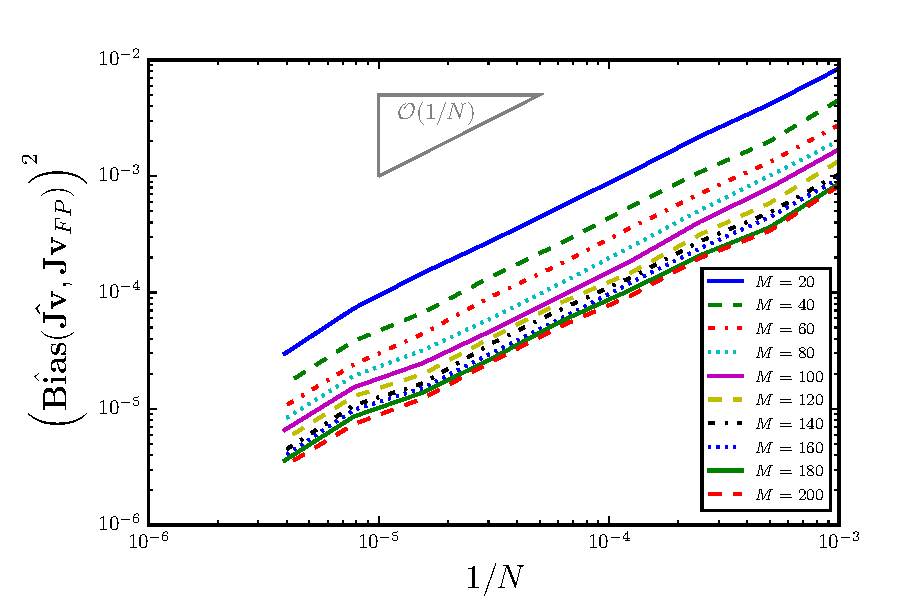
\includegraphics[width=14.5cm]{../Problems/WeightedParticles/checkSystem/plots/Bias_Jv_N_M.pdf}
%\caption{The expectation value of the stochastic solution of the Jacobian-vector-product is calculated by averaging over $M$ stochastic realizations. The estimated bias between this solution and the deterministic one is squared and plotted as a function of the number of particles $N$ for different values of $M$.  For large particle numbers, the estimated bias becomes independent of $M$ and converges to the real bias. This real bias is the numerical error in the solution of the PDE [Need to check this last statement].}
%\label{Bias_Jv_N_M}
%\end{figure}
%
%
%\begin{figure}
%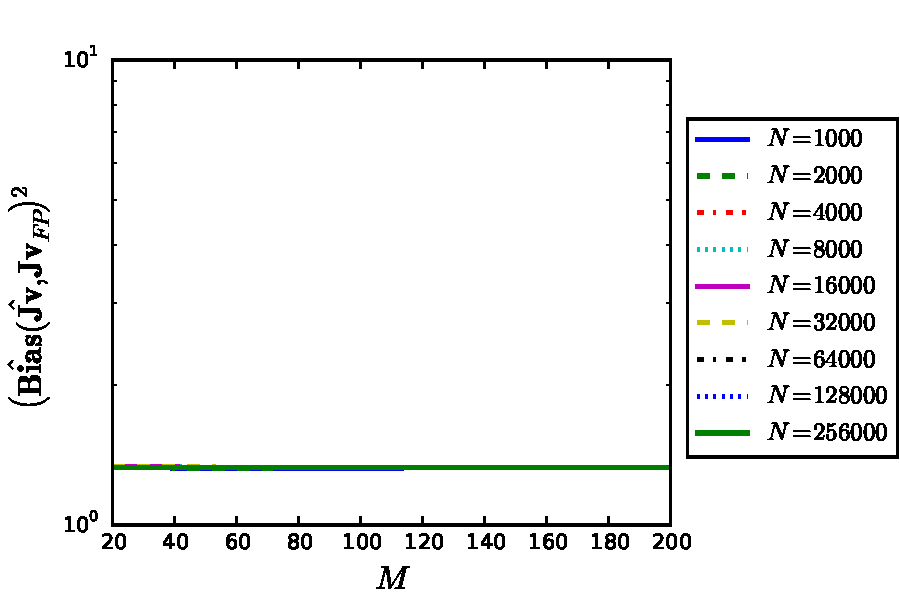
\includegraphics[width=14.5cm]{../Problems/WeightedParticles/checkSystem/plots/Bias_Jv_M_N.pdf}
%\caption{The expectation value of the stochastic solution of the Jacobian-vector-product is calculated by averaging over $M$ stochastic realizations. The estimated bias between this solution and the deterministic one is squared and plotted as a function of the number of realizations $M$ for simulations with different particle number $N$.  For large particle numbers, the estimated bias becomes independent of $M$ and converges to the real bias. This real bias is the numerical error in the solution of the PDE [Need to check this last statement].}
%\label{Bias_Jv_M_N}
%\end{figure}-
%
%\begin{itemize}
%\item
%\end{itemize}
%
%
%%\section{Simulation}
%%\subsection{Default input values}
%%
%%
%%\begin{itemize}
%%\item $\varepsilon  =10^{-5}$
%% \item $ N =10 000$
%%\end{itemize}
%






\section{Method}
\subsection{Coarse time stepper}


To simulate the time evolution of  the density $\U(t)$, we construct  a coarse time stepper $\cts$ which allows the performance of time-steps at the macroscopic level, using only the stochastic simulation of the position vectors of the $N$ particles at the microscopic level, %$\mathbf{X}(t+ n \Delta t)$, 
generated by eq. \eqref{Euler-Mar}. 

To achieve this, we will define two operators (lifting in subsection \ref{section:lifting} and
restriction in subsection \ref{section:restriction}) that relate the microscopic and macroscopic levels of description.
Once these lifting $\mathcal{L}$ and restriction  operators $\mathcal{R}$ have been constructed, a coarse time-stepper $\cts$ 
to evolve the macroscopic state $\U$ over a time interval of length $n \Delta t$ is constructed as a three-step-procedure (lift–evolve–restrict):

\begin{equation}
\U(t + n \Delta t) = \cts(\U) = (\mathcal{R} \circ \mathcal{E}(n \Delta t) \circ  \mathcal{L}(\mathbf{\omega})  ) (\U(t))
\end{equation}
where $\mathcal{E}(n \Delta t)(\U(t))$ is the simulation of the SDE for $N$ particles over $n$ timesteps.


\subsubsection{Lifting: $\U \rightarrow \mathbf{X} $} \label{section:lifting}
Given the density \U, we need to sample a position vector $X_i$ for every particle $i \leq N$. We compute $X$ from a $N$-dimensional vector $\bf{U}$  with uniform random elements $U_i \in [0,1]$ such that $\U(X_i)=U_i$, using the inverse transformation method. The particle does not only gets an inital position, but also a seed for generating random steps in the simulation.

\subsubsection{Restriction:  $\mathbf{X} \rightarrow \U $}
\label{section:restriction}
The restriction operator $\mathcal{R}: \mathbb{Q}^N \rightarrow \mathbb{Q}^k$ maps the microscopic state $\mathbf{X}$ (determined by the position vectors of $N$ particles) to a density \U, discretisized in $k$ bins. This is done by counting the number of particles in every bin $\Delta_j$ for $1\leq j \leq k$: %= x_{j+\frac{1}{2}}-x_{j-\frac{1}{2}}$. 

\begin{equation}
\frac{1}{N} \sum_{i=1}^{N}  w^i \cdot \chi_{\Delta_j}(X^i) = \rho_j  \label{restriction}
\end{equation}
with 
\begin{equation}
\chi_{\Delta_j}(X) = \begin{cases}
  1 & \mbox{if } X \in \Delta_j, \\
  0 & \mbox{if } X \notin \Delta_j. \\
\end{cases}
\end{equation}
%\begin{equation}
% \frac{1}{k}\sum_{j=1}^{k} \rho_j =  \frac{1}{N} \sum_{i=1}^{N}  w_i x_i
%\end{equation}
and setting all weights $w_i =1 $ for $1\leq i \leq N$.

The reason why we explicitly introduced these weights in the restriction operator will be clarified in section \ref{Jv_approx} where we will need to evaluate  the coarse time stepper  $\cts (\U + \varepsilon \mathbf{v})$, now applied to the density shifted with a certain perturbation $\varepsilon \mathbf{v}$. %We explicitly introduced these weights in the restriction operator \eqref{restriction} because they can help to reduce the variance in the jacobian-vector-products. In the finite difference approximation we need to evaluate $\cts (\U + \varepsilon \mathbf{v})$, the coarse time stepper applied to the density shifted with a certain perturbation.
%For the weighted restriction operator, we choose different weights $w_i$ for every particle. (we only use this for calculating the jacobian-vector-produ cts. (Why? Well, the weights are just one if we dont use a perturbation)f
To evaluate the perturbated restriction-operator we will use the weights $ w^i_{\varepsilon}$, determined such that
\begin{equation}
\frac{1}{N} \sum_{i=1}^{N}  w^i_{\varepsilon} \cdot \chi_{\Delta_j} (X^i) = \rho_j + \varepsilon v_j . \label{restriction_eps}
\end{equation}
We do this by computing the weight per bin as $ w^j_{\varepsilon} = 1+ \frac{\varepsilon v_j}{\rho_j}$ and assign this value to each particle in $\Delta_j$. So, small perturbations on the density lead to small perturbations in the weights. The advantage of this weighted restriction operator lies in the possibility to use the same realizations $\mathbf{X}$ in the unperturbated \eqref{restriction} and the perturbated  \eqref{restriction_eps} restriction-operator.



\subsection{Newton-Krylov solver} \label{sec:Newton-Krylov}


If we want to compute steady states for the density $\U_*$ without direct simulation, we can find them by solving the non-linear system

\begin{equation}
  {F}(\U_*) = \U_* - \cts(\U_*) =0. \label{non-linear_system}
\end{equation}
%where $\mathbf{F}$ is nonlinear function from $\R^N$ to  $\R^N$. 
To find the steady state $\U_*$, we apply Newton's method to eq. \ref{non-linear_system}. Starting from an initial state $\U^0$, we iterate %in two  steps, because the inverse of the the inverse of the Jacobian is computationally expensive)
\begin{eqnarray}
\begin{cases}
& \texttt{Solve         }  J(\U^n) \boldsymbol{\delta_n}  =  - {F}(\U^n) \label{linear_system}        \\          
& \texttt{Set     } \U^{n+1} = \U^n+ \boldsymbol{\delta_n} 
\end{cases}
\end{eqnarray}
until convergence. 
$J(\U^n) =   F'(\U^n)  $ denotes the system Jacobian. Each Newton iteration $n$ thus involves evaluating the Jacobian of the timestepper $J(\cts(\U))$.
Since we do not have an explicit formula for $J(\cts)$, we are forced to use an iterative method, such as GMRES, that only requires Jacobian-vector products. %the action of the jacobian times a  vector
%$J(\cts)$, we are forced to use an iterative method, such as GMRES, that only requires Jacobian-vector products.
 \cite{Brown_Krylov}.
The Jacobian $J(\cts)$ applied to a vector $\mathbf{v}$ (with unit norm) will be estimated by a finite difference approximation
\begin{eqnarray}
\label{Jv_approx}
J(\cts) \cdot \mathbf{v} &\approx& \frac{\cts (\U + \varepsilon \mathbf{v}, \boldsymbol{\omega_1} )  - \cts (\U, \boldsymbol{\omega_2})}{\varepsilon} \\
&\approx & \frac{\cts (\U, \boldsymbol{\omega_1} )  + \varepsilon J(\cts) (  \U, \boldsymbol{\omega_1})  \cdot \mathbf{v}  - \cts (\U, \boldsymbol{\omega_2}) }{\varepsilon} \nonumber
\end{eqnarray}

\subsubsection{Analysis of GMRES} \label{GMRES}

The $k$th GMRES iteration minimizes the residual $r= $ over $x_0$ + $\mathcal{K}_k$, where $x_0$ is the initial iterate and $\mathcal{K}_k$ is the the $k$th Krylov subspace
$\mathcal{K_k} = \texttt{Span} \{ r_0, J \cdot r_0, . . . , J_{k-1} \cdot r_0 \}$.
Clearly, (fast) matrix-vector products play a crucial role in generating this sequence since each subsequent vector in the sequence is obtain from the previous one by multiplication by $A$.

\subsubsection{experiments}
For $N=1e^6$ particles and $\Delta_T =0.1$: variance and bias becomes lower, for decreasing GMRES-tolerance, until $\epsilon_{GMRES}= 1e-6$, then blow-up was observed.

\begin{figure}
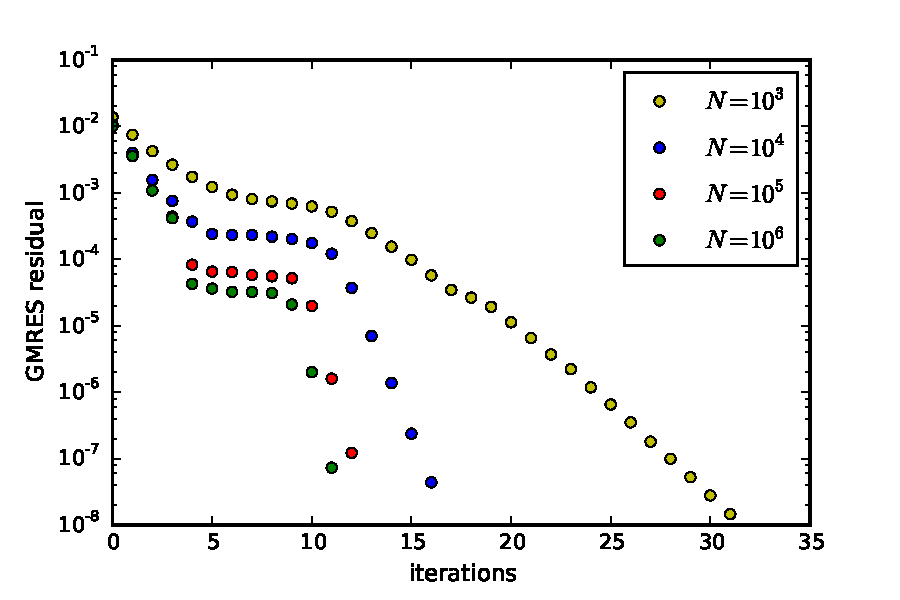
\includegraphics[width=0.5\linewidth]{../Problems/WeightedParticles/checkSystem/plots/GMRES/GMRES_N_Dt_1e-1}
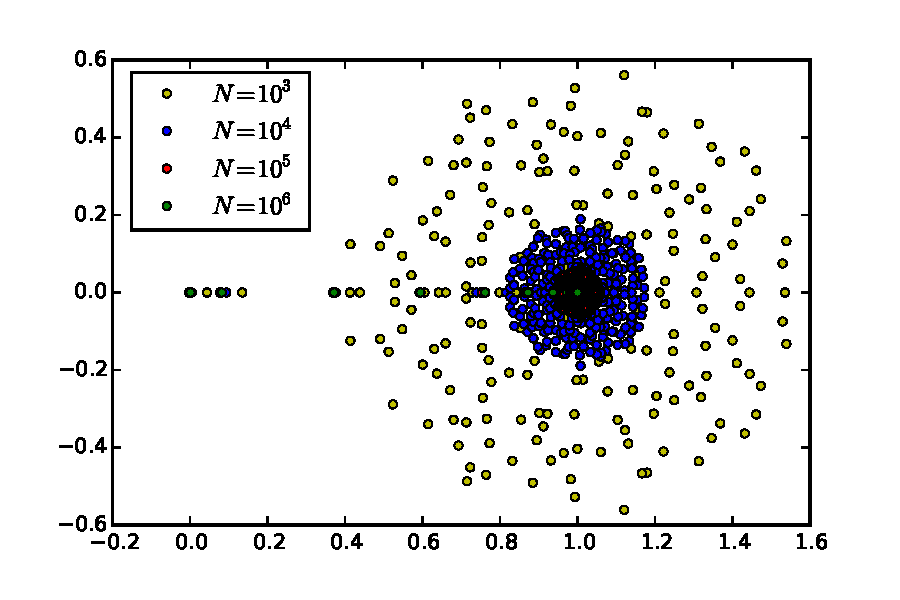
\includegraphics[width=0.5\linewidth]{../Problems/WeightedParticles/checkSystem/plots/GMRES/Spectrum_Dt_1e-1}
\caption{
\textit{Left:} The linear iterations necessary to
obtain convergence decrease as we increase the number of particles  $N$.
\textit{Right:} The linear iterations necessary to
obtain convergence depends on the spectrum of the eigenvalues of the Jacobian. The clustering radius $\rho$ decreases as we increase the number of particles  $N$.
} 
\label{fig:Spectrum_Dt_1e-1}
\end{figure}



To get a better understanding of the convergence behaviour of the GMRES-method, we refer to the following theorem.
\begin{Theorem}[Proof in \cite{broyden2004krylov} and \cite{campbell96}]
Let $ \mathbf{A} \in \mathbb{C}^{n\times n}$ and assume it has $m$ distinct eigenvalues $\lambda_i$ clustered so that for some $\rho > 0 $ and $z \in \mathcal{C}$ , $|\lambda_i - z| \leq \rho$, together with $p$ eigenvalues $\mu_i$ (outliers), each of multiplicity $m_j$ and each lying outside the cluster $|\mu_i - z| > \rho$. Let $d= \sum_{j=1}^p m_j$  so that $n= d+m$. Then, if GMRES is applied to a set of equations with such a matrix of coefficients, it follows, for $k>0$,

\begin{equation}
\| \mathbf{r}_{d+k+1} \| \leq C  \left( \frac{\rho}{|z|} \right)^k  \| \mathbf{r}_1 \| ,
\end{equation}
where $C$ is a constant not depending on $k$.
\end{Theorem}

The theorem states that GMRES may behave as if it were a two-stage process. In the first phase the terms due to the outliers are eliminated before rapid linear convergence sets in for the second phase. The rate of convergence in this second stage is determined by $\frac{\rho}{\lvert z\lvert}$, where $z$ represents the center of the cluster and  $\rho$ its radius. The closer $z$ is to the origin, the slower the expected convergence of the algoritm. If the radius of the cluster $\rho$ is small, we expect a faster convergence of the algorithm. This is observed in figure \ref{fig:Spectrum_Dt_1e-1}.




\subsection{Variance reduced Jacobian-vector products}

If we use the solution of the PDE, eq. \eqref{pde_discretization}, the time stepper is deterministic and the calculation of the Jacobian-vector products is straightforward. If we use the solutions of the SDE however, we have to deal with numerical noise in evaluating eq. \ref{Jv_approx}.
Because the coarse time-stepper is stochastic, repeating $\cts$ with two sets of random numbers ($\boldsymbol{\omega_1}$ and $ \boldsymbol{\omega_2}$)  will give different results. For $ \varepsilon \ll 1$ this will result in an $\mathcal{O}(1/(\varepsilon^2 N))$ variance. Consequently the variance on the Jacobian-vector-products will grow unboundedly as $\varepsilon$ tends to zero and $J(\cts) \cdot \mathbf{v}$ completely loses the structure of the perturbation \V.

This numerical noise can be reduced by using the same random numbers $\boldsymbol{\omega}$ for the unperturbed and perturbed simulations. If we apply the weighted restriction operator \eqref{restriction_eps},  we get the same microscopic realizations in the lifting step - the only difference is in the computation of the weights. As such,  we impose $\boldsymbol{\omega_1} = \boldsymbol{\omega_2}$ in eq. \eqref{Jv_approx} and consequently the variance of $J(\cts) \cdot \mathbf{v}$ is bounded and of  $\mathcal{O}(1/ N)$.  In the limit of infinitely many particles, the result will converge to the exact Jacobian-vector product. For finite values of $N$, there will be noise in the Jacobian-vector product as a result of the random selection of a subset of all possible realizations. The presented procedure only prevents noise blowup that would arise if a different selection of realizations were considered for the perturbed and unperturbed coarse time-step.


\section{Analysis}
\subsection{Variance}

Fig. \ref{Var_N} shows that the variance on the stochastic solution for the Jacobian-vector-product converges to zero with $\mathcal{O}(1/ N)$ and that it does not depend on the value of $\varepsilon$.

\begin{figure}
\centering
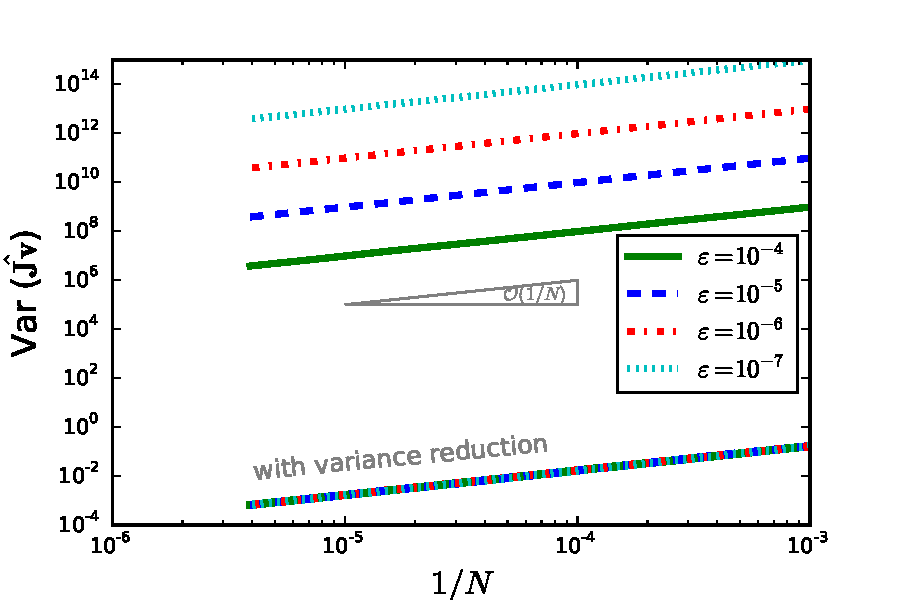
\includegraphics[width=0.8\linewidth]{../Problems/Particles/checkSystem/plots/Var_N_eps_nw}
\caption[Effect of variance reduction]{In the case of unweighted restriction, the variance on the stochastic solution of the Jacobian-vector-product becomes unbounded as we decrease the perturbation size $\epsilon$. By using weights in the restriction step, the variance does not longer depend on the value of $\varepsilon$ and   converges to zero with $\mathcal{O}(1/ N)$.}
\label{Var_N}
\end{figure}

%\subsubsection{Analysis of GMRES} \label{GMRES}

The $k$th GMRES iteration minimizes the residual $r= $ over $x_0$ + $\mathcal{K}_k$, where $x_0$ is the initial iterate and $\mathcal{K}_k$ is the the $k$th Krylov subspace
$\mathcal{K_k} = \texttt{Span} \{ r_0, J \cdot r_0, . . . , J_{k-1} \cdot r_0 \}$.
Clearly, (fast) matrix-vector products play a crucial role in generating this sequence since each subsequent vector in the sequence is obtain from the previous one by multiplication by $A$.

\subsubsection{experiments}
For $N=1e^6$ particles and $\Delta_T =0.1$: variance and bias becomes lower, for decreasing GMRES-tolerance, until $\epsilon_{GMRES}= 1e-6$, then blow-up was observed.

\begin{figure}
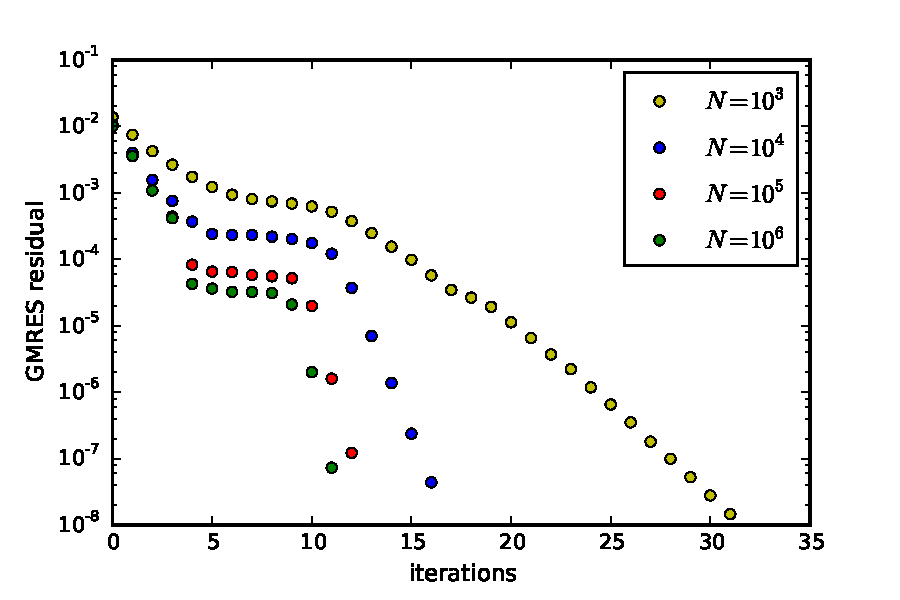
\includegraphics[width=0.5\linewidth]{../Problems/WeightedParticles/checkSystem/plots/GMRES/GMRES_N_Dt_1e-1}
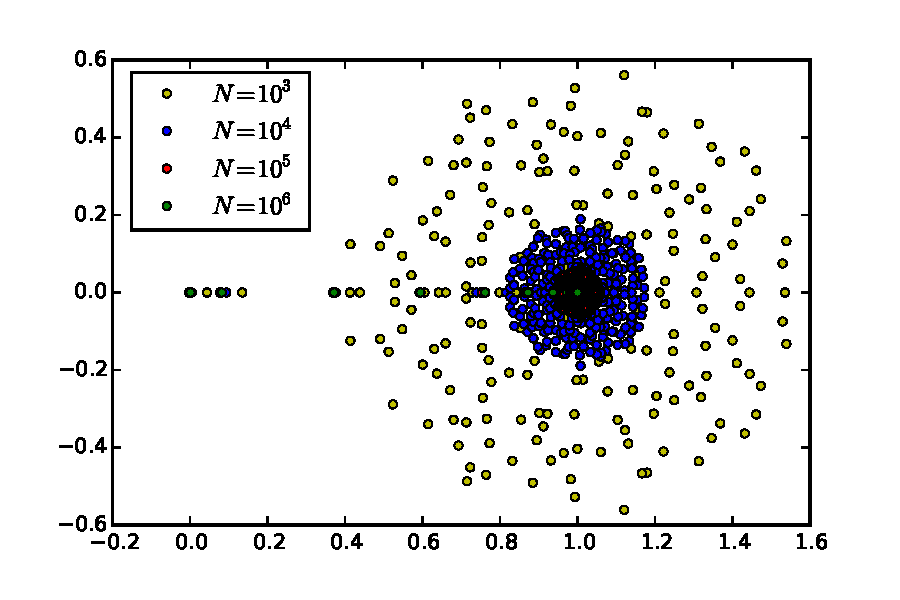
\includegraphics[width=0.5\linewidth]{../Problems/WeightedParticles/checkSystem/plots/GMRES/Spectrum_Dt_1e-1}
\caption{
\textit{Left:} The linear iterations necessary to
obtain convergence decrease as we increase the number of particles  $N$.
\textit{Right:} The linear iterations necessary to
obtain convergence depends on the spectrum of the eigenvalues of the Jacobian. The clustering radius $\rho$ decreases as we increase the number of particles  $N$.
} 
\label{fig:Spectrum_Dt_1e-1}
\end{figure}



To get a better understanding of the convergence behaviour of the GMRES-method, we refer to the following theorem.
\begin{Theorem}[Proof in \cite{broyden2004krylov} and \cite{campbell96}]
Let $ \mathbf{A} \in \mathbb{C}^{n\times n}$ and assume it has $m$ distinct eigenvalues $\lambda_i$ clustered so that for some $\rho > 0 $ and $z \in \mathcal{C}$ , $|\lambda_i - z| \leq \rho$, together with $p$ eigenvalues $\mu_i$ (outliers), each of multiplicity $m_j$ and each lying outside the cluster $|\mu_i - z| > \rho$. Let $d= \sum_{j=1}^p m_j$  so that $n= d+m$. Then, if GMRES is applied to a set of equations with such a matrix of coefficients, it follows, for $k>0$,

\begin{equation}
\| \mathbf{r}_{d+k+1} \| \leq C  \left( \frac{\rho}{|z|} \right)^k  \| \mathbf{r}_1 \| ,
\end{equation}
where $C$ is a constant not depending on $k$.
\end{Theorem}

The theorem states that GMRES may behave as if it were a two-stage process. In the first phase the terms due to the outliers are eliminated before rapid linear convergence sets in for the second phase. The rate of convergence in this second stage is determined by $\frac{\rho}{\lvert z\lvert}$, where $z$ represents the center of the cluster and  $\rho$ its radius. The closer $z$ is to the origin, the slower the expected convergence of the algoritm. If the radius of the cluster $\rho$ is small, we expect a faster convergence of the algorithm. This is observed in figure \ref{fig:Spectrum_Dt_1e-1}.





The convergence of the density to the real solution, strongly depends on the number of particles $N$ and on the choice of $\epsilon$ in the GMRES-method. 



\subsection{}



\subsection{bias}


\section{Application: Systemic Risk}

%\subsection{Including an interaction term}

Until now, we considered a system of non-interacting particles. We will now extend our model to a mean field model by introducing a third parameter $\alpha$, which is the degree of interaction or cooperation in the system. A simple form of cooperative behaviour is the case where each agent tends to follow the state of the majority (or, each particle feels an attractive force towards the mean state of the system). To include this cooperation effect in our stochastic simulation, we add this mean reversion term to the SDE \eqref{SDE}:

\begin{equation} 
\label{SDE_meanfield}
    \dd x = \mu V(x) \dd t + \sigma  \dd{W_t} + \alpha(\bar{x} -x) \dd t ,
\end{equation}
with  $\bar{x}(t) = \frac{1}{N} \sum_{i=1}^{N} x_i(t)$ denoting the empirical mean. 


An interesting application of this model to banks and insurance is the emergence of systemic risk.  Banks will try to minimize their own individual risk by spreading the risk between each other. However, this may increase the risk that they may all fail: reducing individual risk on a micro-scale can increase systemic risk on a macro-scale. 
Garnier, Papanicolaou and Yang already made use of the dynamics in eq. \eqref{SDE_meanfield}  to show that interconnectedness between agents indeed affects the stability of the whole system, causing systemic risk  \cite{Garnier}. They defined $x_i$  as the state of risk of agent $i$. The bi-stable-state structure of the potential $V(x)$ ensures that each risk variable stays around $-1$ (defined as the normal state) or $+1$ (the failed state).  A natural measure of systemic risk is then the transition probability of the empirical mean $\bar{x}$ from the normal state to the failed state. 
 

To establish the idea, let us repeat the numerical simulations with eq. \ref{SDE_meanfield}. The evolution of the system is now characterized by  by the initial conditions, the three parameters ($\mu$, $\sigma$, $\alpha$) and by the system size $N$. Figure \ref{fig:sysrisk}  illustrates the behaviour of the empirical mean $\bar{x}$. The simulations were performed with all agents initially in the normal state. Nevertheless, if randomness dominates the interaction, the agents can move immediately to the other potential well. The system then behaves like $N$ independent diffusions, and hence, by the symmetry of the potential, the mean state will be attracted to a single mixed state $\bar{x}=0$. Upon increasing the interaction parameter $\alpha$, however, we find two new macroscopic states, suggesting the precence of a pitchfork bifurcation at the macroscopic level. These solutions are no stable steady states, but rather coarse metastable states. Their lifetime is linked to the finite system size. 



\begin{center}
\begin{figure}
\includegraphics[width=0.5\textwidth]{../../riskmodel/Problems/WeightedParticles/checkSystem/plots/xmean_alpha1}
\includegraphics[width=0.5\textwidth]{../../riskmodel/Problems/WeightedParticles/checkSystem/plots/xmean_alpha5}

\caption{The empirical mean, simulated for different $\alpha$. \textit{Left}: the system has one single state $\bar{x}=0$. \textit{Right}: for $\alpha> \alpha_c$ two metastable equilibria emerge. 
 The red dashed lines are approximated  analytical solutions for the steady states. \label{fig:sysrisk}}
\end{figure}
\end{center}


 \begin{center}
\begin{table}
\caption{Parameter values}
  \begin{tabular} { | c  c | c |}    \hline   
     %FTCS-scheme  &   Euler-Maruyama-scheme  \\  
   \textit{ {Discretization parameters}}&    &  SDE    \\ \hline
    Discretization step  & $\Delta x $  & $10^{-2}$ \\ 
        Number of discretization steps  & $n_x$ &  340 \\ 
    Time step  &  $\Delta t$ &   $10^{-2}$ \\ 
       Number of timesteps  & $n$  &  $10^{6}$ \\ \hline
  \end{tabular}
%\quad
%     \begin{tabular}  { | c | c | c |  }  \hline
%     \multicolumn{3}{|c|} {\textit{ System parameters}   }    \\
%    \hline  
%    Diffusion coefficient  & $D $ & $0.5$ \\ 
%   Drift coefficient &  $\mu$ & $ 1$ \\ \hline
%  \end{tabular}
\end{table}
\end{center}

\subsection{Bifurcation study}



\subsubsection{Nota's}
Tijdens elke continueringsstap, wordt een nieuw punt gecreëerd dat initieel de dichtheid \U krijgt van het vorig punt en met een parameter (D) die horizontaal word geupdate. Dan wordt de norm van het residu berekend $\norm{ \U(t) - \U(t+\Delta t)} $, waarin de dichtheid op de volgende tijdsstap verkregen wordt door een simulatie van het systeem met de nieuwe parameter. De grootte van het residu is dus afhankelijk van de stapgrootte in de bifurcatieparamter. De newtontolerantie is de norm van het residu. Als de newton-tolerantie te groot gekozen wordt (in vergelijking met de stapgrootte van het residu), dan wordt er geen Newton-iteratie uitgevoerd. Als de Newton-tolerantie evenwel te klein gekozen wordt, dan bereikt de Newton-solver mogelijk geen convergentie ten gevolge van de ruis. De Newton-tolerantie moet dus weloverwogen gekozen worden. 



\subsection{Results for the pde}
Ook hier zien we dat de keuze van de newtontolerantie belangrijk is (te groot = kans op dezelfde toestanden , te klein= failed iterations).
Dit kan echter opgevangen worden door de oplossing van dx nauwkeuriger te maken door de tolerantie van de GMRES te verfijnen (het probleem was dat er dx=0 oplossingen werden teruggegeven) 

\begin{figure}
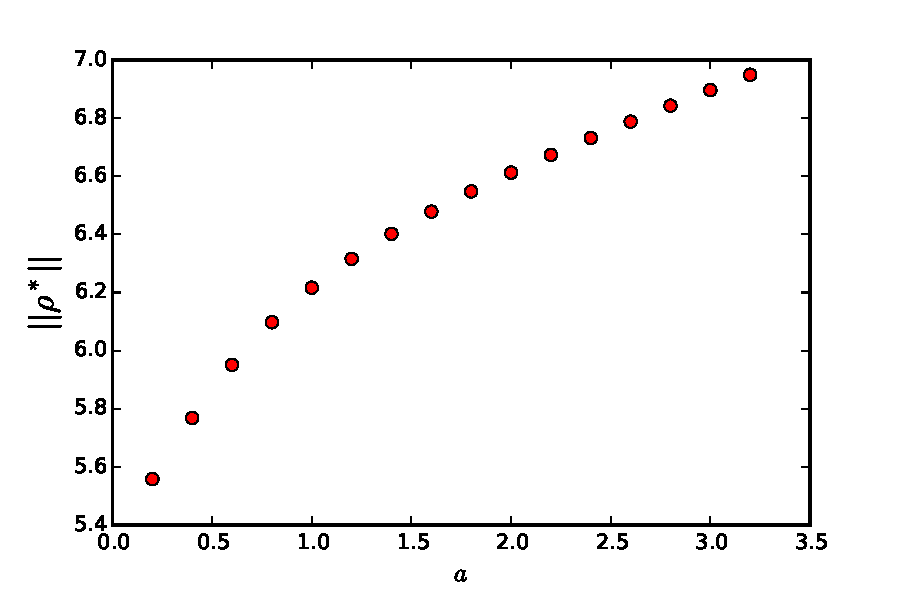
\includegraphics{../Problems/WeightedParticles/checkSystem/plots/bifurcation_pde(D)}
\caption{  Bifurcation diagram of the steady states calculated with the Newton-Krylov-Solver for the PDE. $\Delta t = 10^{-4}, \Delta T = 10^{-2}, \Delta x = 10^{-2}, \Delta D = 0.01, \epsilon_{GMRES}=10^{-5},  \delta_{Newton} = 10^{-7}, \epsilon=10^{-5}$
}
\end{figure}

\subsection{Results for the sde}
We chose $\Delta \sigma = 0.05$ as continuation step seize. Performing a bifurcation with smaller steps is pointless, because the difference in densities will become too small in comparison with the noise on the residual.

\begin{figure}
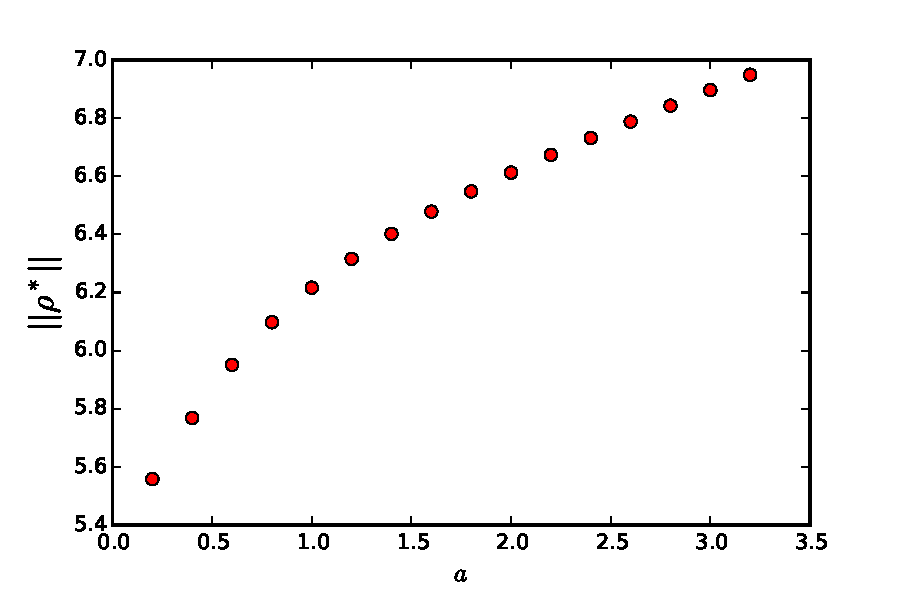
\includegraphics{../Problems/WeightedParticles/checkSystem/plots/bifurcation_pde(D)}
\caption{  Bifurcation diagram of the steady states calculated with the Newton-Krylov-Solver for the SDE. $\Delta t = 10^{-3}, \Delta T = 10^{-1}, \Delta x = 10^{-2}, \epsilon_{GMRES}=10^{-5},  \delta_{Newton} = 10^{-7}, \epsilon=10^{-5}$
}
\end{figure}

%\begin{center}
%\begin{table}
%\caption{Parameter values}
%  \begin{tabular} { | c  | c |}    \hline   
%     %FTCS-scheme  &   Euler-Maruyama-scheme  \\  
%   \textit{ {Discretization parameters}}&    &  SDE    \\ \hline
%       $\Delta t $  & $10^{-4}$ \\ 
%       $\Delta T $ &  $10^{-2}$ \\ 
%      $ \Delta x &  $10^{-2}$ \\ 
%       $ \Delta D$  $  &  $ 0.01 $ \\ \hline
%  \end{tabular}
%\end{table}
%\end{center}

\subsubsection{Calculating fixed points}
The steady  states are computed with the Newton-Krylov solver described in section \ref{sec:Newton-Krylov} and compared with the approximated analytical solutions, calculated by Garnier et. al for small $h$ \cite{Garnier}.



\begin{center}
\begin{figure}
\includegraphics[width=1\textwidth]{../../riskmodel/Problems/WeightedParticles/checkSystem/plots/steady_states.pdf}
\caption{\label{fig:bif_anal}}
\end{figure}
\end{center}



\subsubsection{Continuation}
We use a pseudo-arclength contunaution method with secant prediction steps.
In fig. \ref{todo} we show a bifurcation diagram of the densities. 





\begin{center}
\begin{figure}
\includegraphics[width=0.8\textwidth]{../../riskmodel/Problems/WeightedParticles/checkSystem/plots/bif_alpha}
\caption{\label{fig:bif_anal}}
\end{figure}
\end{center}




%\begin{equation}
%\xi = sqrt(1-3*C)*(1+ 6*mu/(sigma**2)*C**2*(1-2*C)/(1-3*C))
%\end{equation}  
%
%


By adding the mean reversion term, the Fokker-Plack equation \eqref{fokkerplanck}  describing the evolution of the density, now becomes

\begin{equation}
\label{fp_mean_field}
\pa{\rho(x,t)}{t} = - \mu \pa{( V(x) \rho(x,t))}{x} - \alpha \pa{}{x} \left[ \left(\int x \rho(x,t) \mathrm{d}x  -x \right) \rho(x,t) \right] + \frac{\sigma^2}{2}  \ppa{\rho(x,t)}{x} .
\end{equation}

Explicit solutions of eq. \label{fp_mean_field} are not available in general, but we can find equilibrium solutions. Assuming 





\section{Convergence of the Newton Method}



We show some numerical experiments that show how the Newton method converges to the fixed point. 

\subsection{Maximal accuracy}


\subsubsection{Estimating stopping criterion for the non-linear solver}
The accuracy on the Newton-Krylov solution is inevitably limited by the noise on the stochastic coarse-time-stepper, which appears in the evaluation of the residual and in the evaluation of the Jacobian-vector-product. The variance on the coarse-time-stepper is of order $\mathcal{O}(\frac{1}{N})$, as shown in fig. \ref{fig:Variance_on_cts(N-1)}. If we use weighted restriction, the variance on the Jacobian-vector-product converges in the same way.  Therefore, the accuracy on the Newton-Krylov solution will depend on the number of particles $N$ used to calculate the coarse time-stepper.  This is confirmed in fig. \ref{fig:Newton_sde_res(k)}, which shows the convergence of the Newton-residuals. When the Newton-Krylov solution is converged, it stays oscillating around the true solution with a standard deviation depending on the number of particles. Because the solution only depends on the previous density and on the random choices in the coarse time stepper, we can interpret this as a Markov chain. The residual averaged out over the converged Newton iterations is a good indication of the best tolerance we can achieve. It converges as $\mathcal{O}(\frac{1}{\sqrt{N}})$. Given the number of particles $N$,  we will use this tolerance as the stopping criterion for the Newton-method.

\subsubsection{Estimating stopping criterion for the linear solver}
Because the solution of the Newton-Krylov solution will contain noise anyway, it is pointless to iterate the linear solver until reaching machine precision.
In fact, for low particle numbers (and a high variance on the left and right side of the linear equation we need to solve), we observe more failed Newton-iterations if the GMRES-tolerance is chosen too small.  A question of interest is then `what is a good value for the GMRES-tolerance?'. The answer depends on the desired accuracy of the calculated fixed points. For instance in fig. \ref{fig:Newton_sde_res(k)_tol1e-4}, we observe that we  can already stop the Krylov iterations if the density is calculated to an accuracy of %$\varepsilon_{\texttt{GMRES}}=
$10^{-4}$ when $N \leq 10^7$, but that we need a smaller GMRES-tolerance if a higher accuracy is desired (by using more particles). Therefore, in the simulations we  will use $\varepsilon_{\texttt{GMRES}}= 10/N$.


\begin{figure}[H!]
\centering
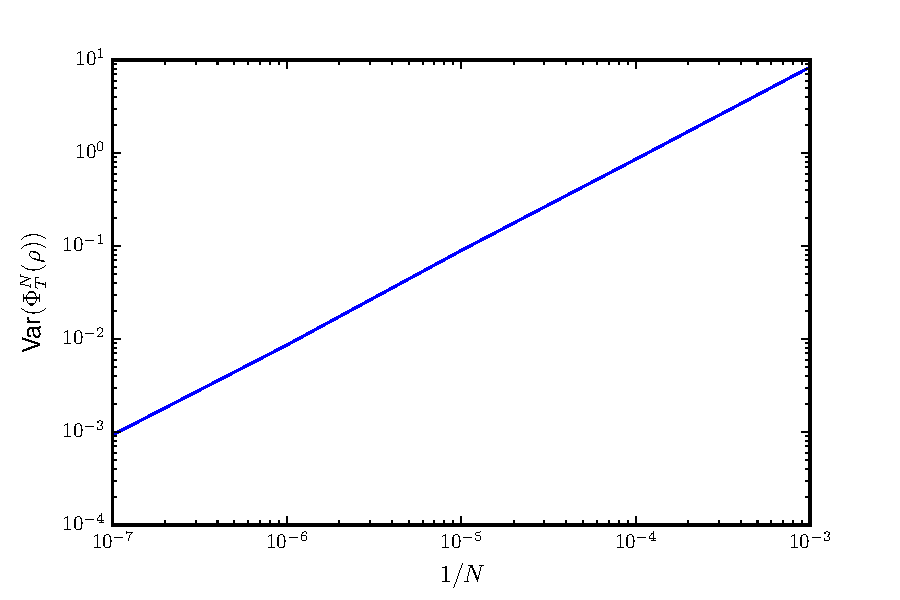
\includegraphics[width=0.49\linewidth]{../Problems/WeightedParticles/checkSystem/plots/Variance_on_cts(N-1)}
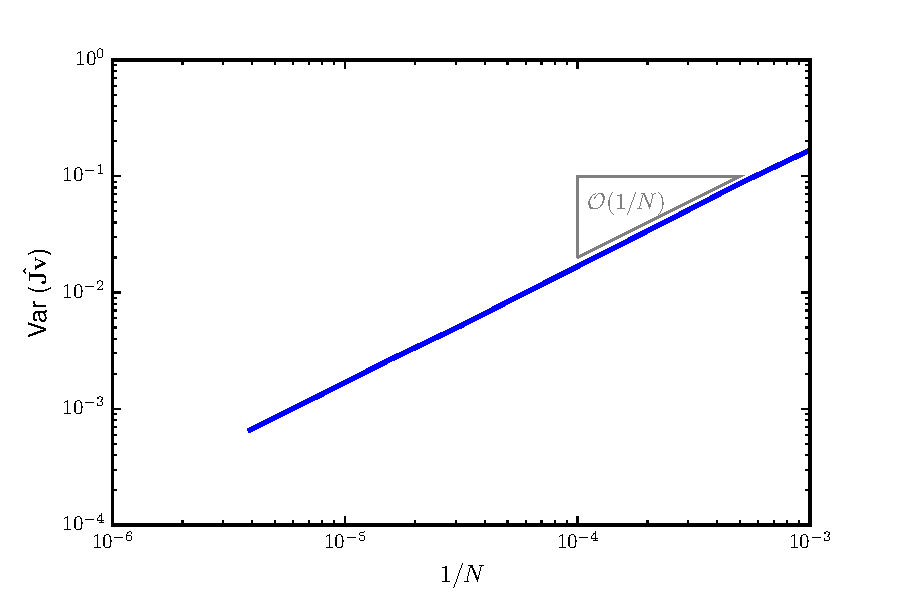
\includegraphics[width=0.49\linewidth]{../Problems/WeightedParticles/checkSystem/plots/Variance_on_Jv}
\caption{The variance of the coarse time-stepper and the variance on the Jacobian vector-product converge to zero with $\mathcal{O}(\frac{1}{N})$ }
\label{fig:Variance_on_cts(N-1)}
\end{figure}



\begin{figure}[H!]
\centering
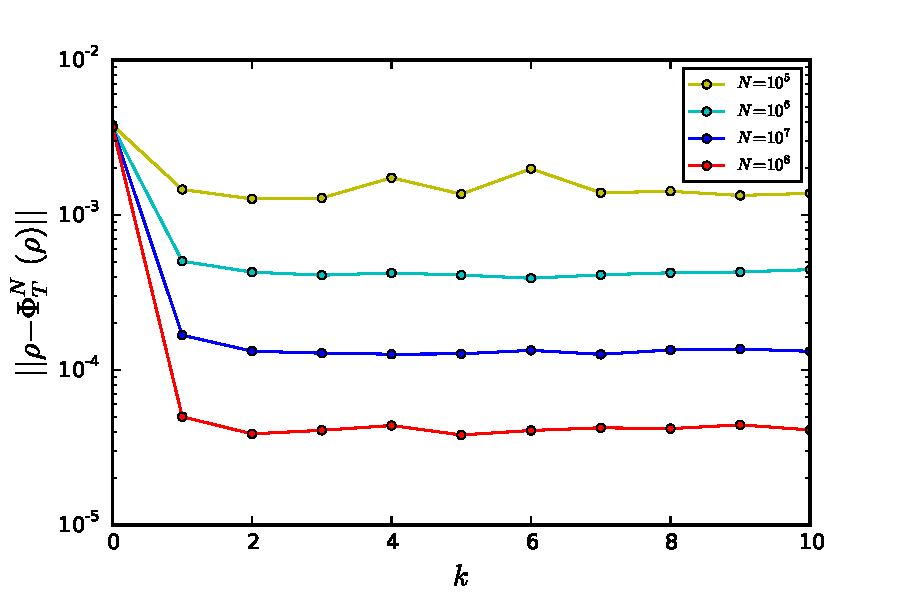
\includegraphics[width=0.5\linewidth]{../Problems/WeightedParticles/checkSystem/Newton/plots/Newton_sde_res(k)_Dt_e-2_tol1e-7.pdf}
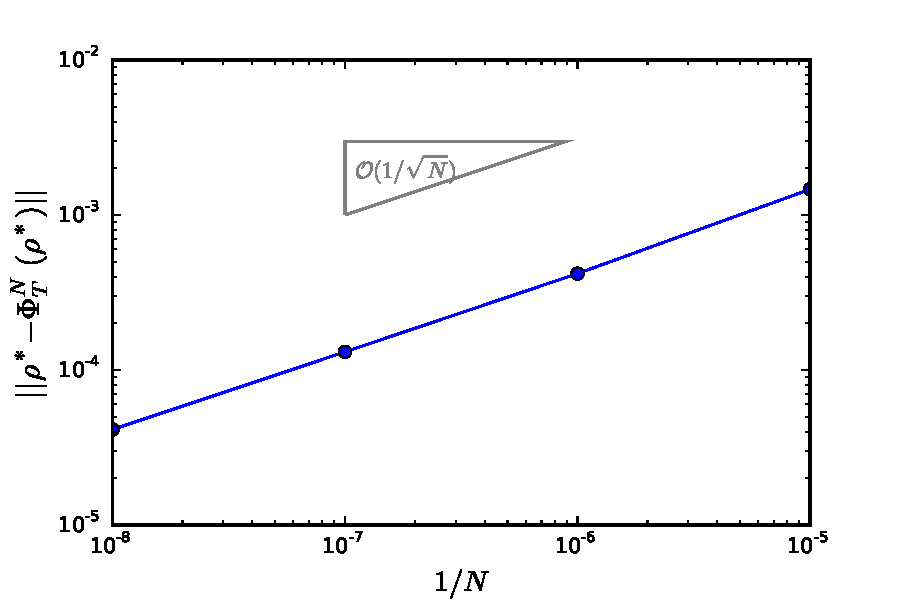
\includegraphics[width=0.49\linewidth]{../Problems/WeightedParticles/checkSystem/Newton/plots/Tolerance_on_NK-solution_converges_N-1_tol_1e-7.pdf}

\caption{ The non-linear solver converges after 1 or 2 Newton iterations, up to a tolerance which depends on the number of particles $N$ (\textit{left}). This best achieved tolerance converges to zero with  $\mathcal{O}(\frac{1}{\sqrt{N}})$ (\textit{right}). Parameter values:  $\Delta t = 10^{-3}, \Delta T = 10^{-1} , \epsilon_{\texttt{GMRES}}=10^{-7}$
}.
\label{fig:Newton_sde_res(k)}
\end{figure}



\begin{figure}[H!]
\centering
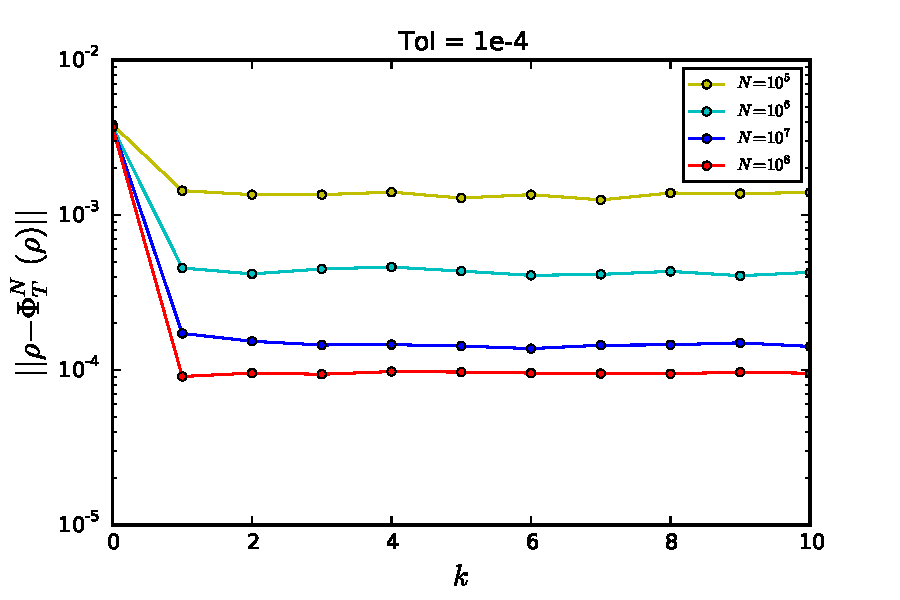
\includegraphics[width=0.5\linewidth]{../Problems/WeightedParticles/checkSystem/Newton/plots/Newton_sde_res(k)_Dt_e-2_tol1e-4}
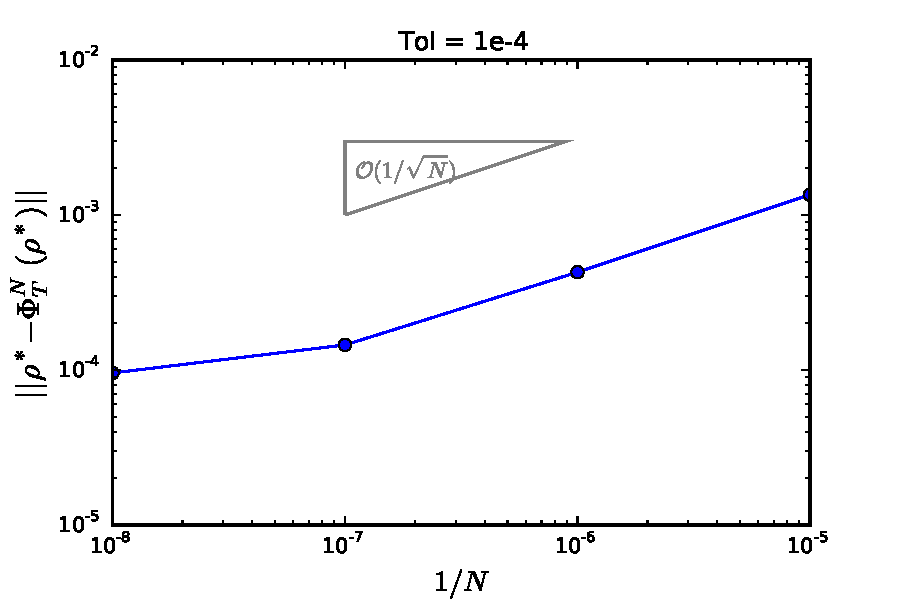
\includegraphics[width=0.49\linewidth]{../Problems/WeightedParticles/checkSystem/Newton/plots/Tolerance_on_NK-solution_converges_N-1_tol_1e-4}

\caption{ The best achieved tolerance for $N=10^8$ is limited because of the size of the GMRES-tolerance ($\epsilon_{\texttt{GMRES}}=10^{-4}$)
}
\label{fig:Newton_sde_res(k)_tol1e-4}
\end{figure}



%How to cheaply estimate the stopping criterion?

%Is the resulting fixed point biased?
%Can we reduce variance by averaging over a number of 'converged' Newton iterations?
%Additional questions of interest:
%
%Can we stop the Krylov iterations before reaching machine precision (knowing that the end result will contain noise anyway)? 
%
%Does an inaccuracy in the solution of the linear systems increase the required number of Newton iterations?
%
%Do we keep the particles fixed throughout the Newton iterations as well? (We can then probably converge the Newton procedure to machine precision.) What is then the probability distribution of the obtained fixed points? Bias? Variance?

%\subsection{Results for the pde}
%Ook hier zien we dat de keuze van de newtontolerantie belangrijk is (te groot = kans op dezelfde toestanden , te klein= failed iterations).
%Dit kan echter opgevangen worden door de oplossing van dx nauwkeuriger te maken door de tolerantie van de GMRES te verfijnen (het probleem was dat er dx=0 oplossingen werden teruggegeven) 

%\begin{figure}
%%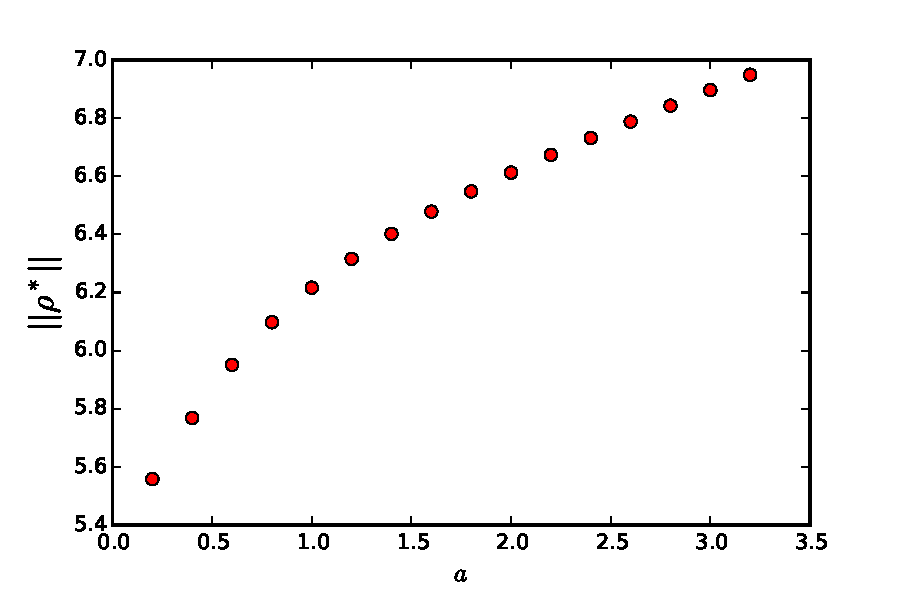
\includegraphics{../Problems/WeightedParticles/checkSystem/plots/bifurcation_pde(D)}
%\caption{  Bifurcation diagram of the steady states calculated with the Newton-Krylov-Solver for the PDE. $\Delta t = 10^{-4}, \Delta T = 10^{-2}, \Delta x = 10^{-2}, \Delta D = 0.01, \epsilon_{GMRES}=10^{-5},  \delta_{Newton} = 10^{-7}, \epsilon=10^{-5}$
%}
%\end{figure}

%\subsection{Results for the sde}


\subsection{Continuation}
 We start from a known solution to the steady-state problem, increment the continuation parameter and solve a new problem using the previous solution as an initial guess. We chose $\Delta \sigma = 0.05$ as continuation step size. Performing a bifurcation with smaller steps is pointless, because the difference in densities will become too small in comparison with the noise on the residual.

\begin{figure}[h]
\centering
%\begin{subfigure}{0.5\textwidth}
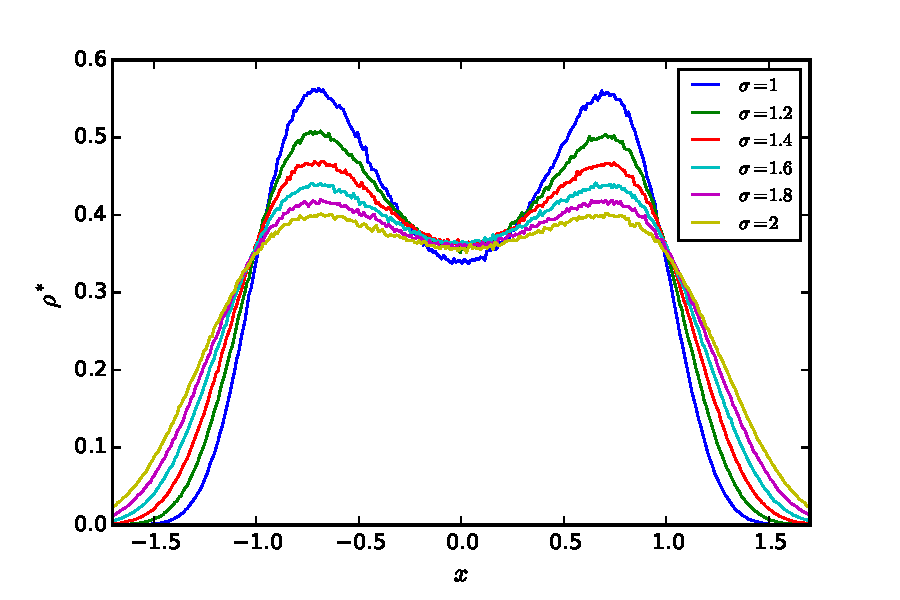
\includegraphics[width=0.49\linewidth]{../Problems/WeightedParticles/checkSystem/plots/bif/fixed_states_sde(sigma)_Ne6_mean_M10_LR}
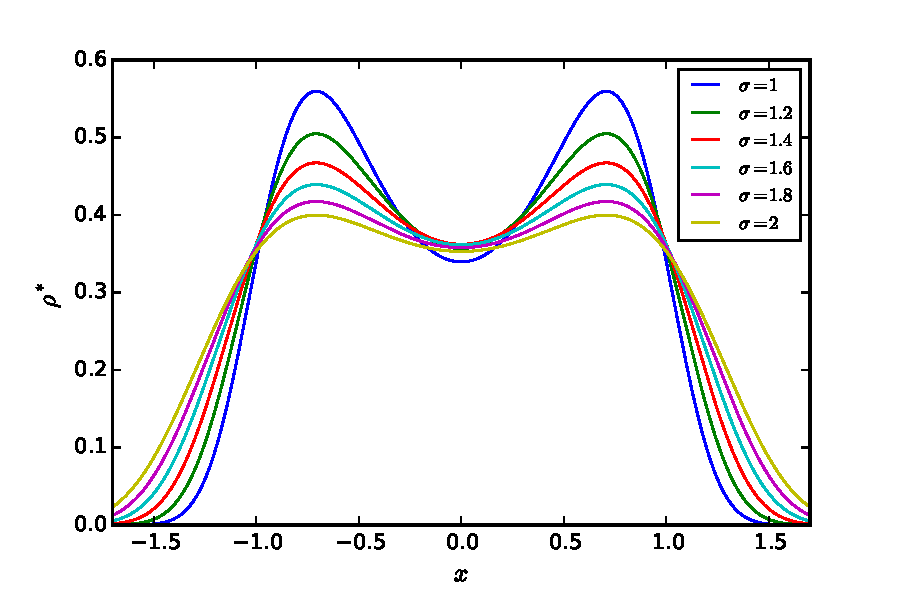
\includegraphics[width=0.49\linewidth]{../Problems/WeightedParticles/checkSystem/plots/bif/fixed_states(sigma)_analytic}
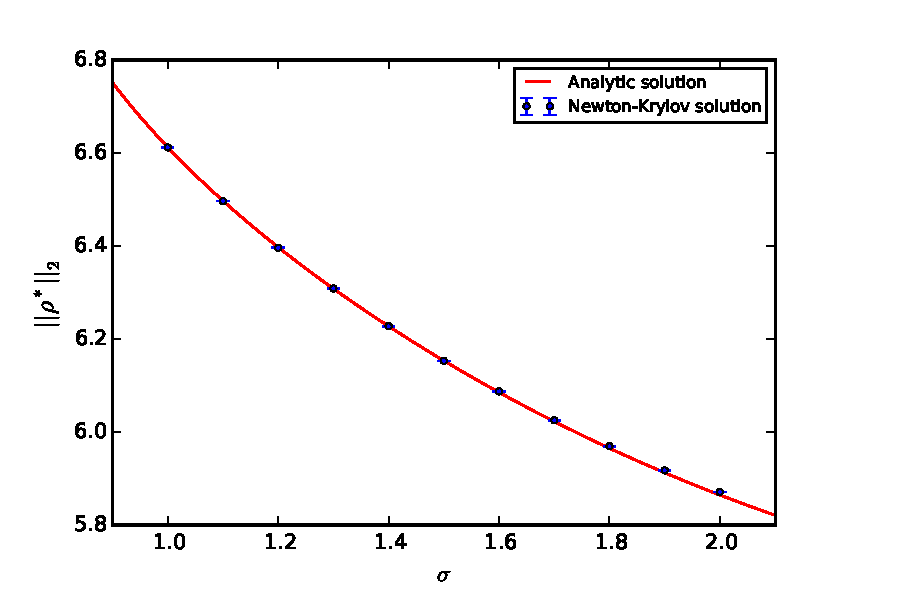
\includegraphics[width=0.9\linewidth]{../Problems/WeightedParticles/checkSystem/plots/bif/bifurcation_sde_Ne6_anal(sigma)_LR}
\caption{The steady states calculated with the Newton-Krylov-solver for the SDE  (\textit{top left}) are compared with the analytical solutions (\textit{top right}). The fixed points are visualized as the 2-norm of the density, and plotted as a function of the continuation parameter $\sigma$ (\textit{bottom}). The branch of fixed points appears to be in correspondence with the 2-norm of the analytic function $\rho^*(\sigma) =  \exp{\left[-\frac{2 V(x)}{\sigma^2}\right]} $. %{\mathcal{N}} $.
Parameter values: $\Delta \sigma =0.1$, $N=10^6$, $M=10$, $\Delta t = 10^{-3}, \Delta T = 10^{-1}, \Delta x = 10^{-2}, \epsilon_{\texttt{GMRES}}=10^{-5},  \delta_{\texttt{Newton}} = 45 \cdot 10^{-5}, \varepsilon_J=10^{-5}$}.
\label{fig:fixed_states_sde(sigma)_Ne6_mean_M10_LR}
\end{figure}





%
%\subsection{timings}
%Simulation time for solving sde, ten Newton iterations, with N=1e8, tol=1e-7: Time = 34u26m15s
%






\bibliographystyle{plain}
\bibliography{biblio.bib}





\end{document}
